\section*{Тестовая функция}
\addcontentsline{toc}{subsection}{Тестовая функция}

В качестве тестовой функции для минимизации
использовалась смещённая функция Растригина $R$:

\begin{equation*}
    r = \sum_{i = 1}^{D}(x_i^2 - 10\cos(2 \pi x_i) + 10)
\end{equation*}

\begin{equation*}
    R = r\left(\frac{5.12 (x - o_r)}{100}\right) + 800
\end{equation*}

Вектор параметров $x$ был выбран размера 30.

Было проведено тестирование
аналогично описанному в разделе
Численные эксперименты,
однако не были получены
статистические различия.
Отсутствие эффекта
от оптимизации может
быть объяснено тем,
что служебные функции
выполняются значительно быстрее.

\begin{figure}[h]
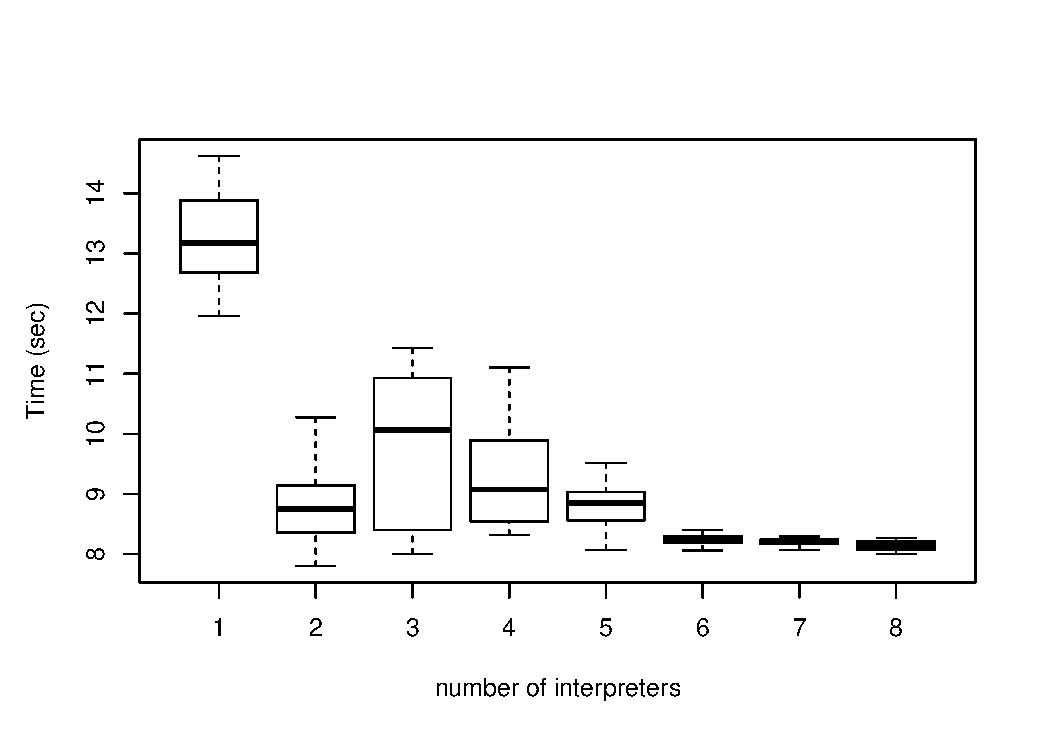
\includegraphics{rastrigin}
\caption{Диаграммы размаха времени исполнения
в зависимости от числа интерпретаторов}
\label{fig:rastriginboxplot}
\end{figure}

На рис.~\ref{fig:rastriginboxplot} видно,
что при увеличение числа интерпретаторов
время выполнения одной и той же задачи
описывает убывающую ветвь гиперболы.

